\begin{frame}
    \frametitle{\problemtitle}

    \begin{itemize}
    \item Given are $1\leq n\leq 10^5$ planets in $3$D space with $\left|x\right|,\left|y\right|,\left|z\right|\leq10^3$.
    \item There are $1\leq m\leq 10^5$ bidirectional straight-line highways
      between pairs of planets.
    \item You can travel over highways by accelerating or decelerating
      at $1\,\textrm{m}/\textrm{s}^2$, taking $1$ litre per second.
    \item You must come to a full stop at the end of each highway.
    \item Answer $1\leq q\leq 10^5$ queries, asking for the minimal amount of
      fuel needed to get to planet $c$ in time at most $1\leq t\leq 10^3$.
    \item If a mission is impossible, output ``\texttt{impossible}''.
    \end{itemize}

    \vspace{0.5em}

    \centering
    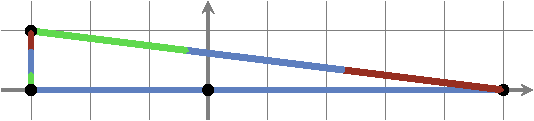
\includegraphics[width=0.8\textwidth]{sample1.pdf}

    \small Illustration of Sample Input 1, showing highways in blue, and a
    route from planet $1$ to planet $3$.
    The green start of a highway indicates acceleration,
    and the red end indicates deceleration.
\end{frame}
